\documentclass[times,usenatbib]{mn2e}
\RequirePackage{graphicx}
\RequirePackage{subfigure}
\RequirePackage{rotating}

\newcommand{\hiir}{H~{\scshape ii}~region}
\newcommand{\hiirs}{H~{\scshape ii}~regions}
\newcommand{\um}{$\mu$m}
\newcommand{\degree}{^{\circ}}
\newcommand{\apj}{ApJ}
\newcommand{\apjs}{ApJS}
\newcommand{\apjl}{ApJL}
\newcommand{\aj}{AJ}
\newcommand{\mnras}{MNRAS}
\newcommand{\pasp}{PASP}
\newcommand{\aap}{A\&A}
\newcommand{\bubblecount}{5,106}

\title[Galaxies in the ZoA]{The Milky Way Project: Galaxies in the Zone of Avoidance\footnote{This publication has been made possible by the participation of more than 40,000 volunteers.}}

\author[Simpson et al.]
{\parbox{\textwidth}{R. J. Simpson$^{1}$\thanks{Email: robert.simpson@astro.ox.ac.uk},
K. Clements$^{2}$,
A. Gazzard$^{3}$,
B. Simmons$^{1}$,
C. J. Lintott$^{1}$}\vspace{0.8cm}\\
\parbox{\textwidth}{
$^{1}$Oxford Astrophysics, Denys Wilkinson Building, Keble Road, Oxford, OX1 3RH, UK \\
$^{2}$Wheatley School, Oxford, UK \\
$^{2}$A. N. Other School, Oxford, UK }}

\date{Draft form \today .}

\pagerange{000--000}

\begin{document}

\label{firstpage}

\maketitle

\begin{abstract}

We present a method for identifying galaxies and protostars through data gathered from the citizen science website `The Milky Way Project�, and report the discovery of 33 previously unknown galaxies in the Zone of Avoidance. 47 candidate galaxies are identified through correlation of markings from volunteers, inspecting Spitzer GLIMPSE and MIPSGAL survey data on `The Milky Way Project' website. The characteristics of these candidate, such as their locations, spectral energy distributions and redshift velocities are used to confirm whether they are galaxies. The magnitudes and integrated flux of the candidates are calculated in GLIMPSE bands 3.6$\mu$m, 4.5$\mu$m, 5.8$\mu$m and 8.0$\mu$m, and MIPSGAL band 24$\mu$m. The velocities of these 33 newly uncovered galaxies appear to correlate with the velocities of over-densities in the large-scale structure, at very low Galactic latitudes either side of the Zone of Avoidance. Our findings therefore suggest that the large-scale structure continues throughout the Zone of Avoidance, and highlight the potential for hundreds more galaxies to be found in far-infrared survey data.

\end{abstract}
\begin{keywords}
H II regions -- infrared: ISM  -- ISM: dust -- stars: formation
\end{keywords}

\section{Introduction}

The Zone of Avoidance (ZoA) remains the missing piece in our map of the large-scale structure of the Universe. Previous studies have shown that careful inspection of far-infrared Galactic plane data (e.g. from the Spitzer Space Telescope) can reveal highly obscured, and thus highly reddened, galaxies in this region \citep{Jarrett+07, Marleau+08}.

\section{The Milky Way Project}
\label{mwp-desc}

The Milky Way Project \citep[MWP,][]{Simpson+12} is the ninth online citizen science project created using the Zooniverse\footnote{http://www.zooniverse.org} platform \citep{2011MNRAS.412.1309S}. The Zooniverse platform supports the activities of all Zooniverse citizen science projects. Built originally for Galaxy Zoo 2 this software, and successive versions of it, have now been used by more than 20 different projects across a range of research disciplines. The Zooniverse toolset is designed primarily as a way to of serving a large collection of `assets' (for example, images or video) to a user interface, and collecting back user-generated interactions with these assets.

Galaxy Zoo \citep{Lintott+08, Lintott+11} and the larger suite of Zooniverse projects have successfully built a large community of volunteers\footnote{Over 750,000 registered volunteers at time of writing.} eager to participate in scientific activities. The Zooniverse has shown that enlisting these `citizen scientists' via the internet is a powerful way to analyze large amounts of data. Human brains excel at pattern recognition tasks, and most people will reach a level of accuracy as high as any expert after a brief introduction. By enlisting citizen scientists, researchers can extend visual classification to large samples of images, having each image examined by a large number of independent classifiers. This allows researchers to tap into the `wisdom of the crowd' effect where the consensus of a group of non-experts is often more accurate than the testimony of a single expert.

Another advantage of enlisting human classifiers is their ability to recognize unusual objects (e.g. galaxies, star clusters, dark clouds in the MWP) which computer search algorithms  may be unable to spot. This has been shown by the serendipitous discovery of Hanny's Voorwerp \citep{2009MNRAS.399..129L} and the case of the Galaxy Zoo `Green Peas' \citep{2009MNRAS.399.1191C}. Spitzer GLIMPSE data is ideally suited to classification by citizen scientists as the amount of data is large and the images contain complex, overlapping structures that are extremely difficult to disentangle using automated algorithms.

\begin{figure}
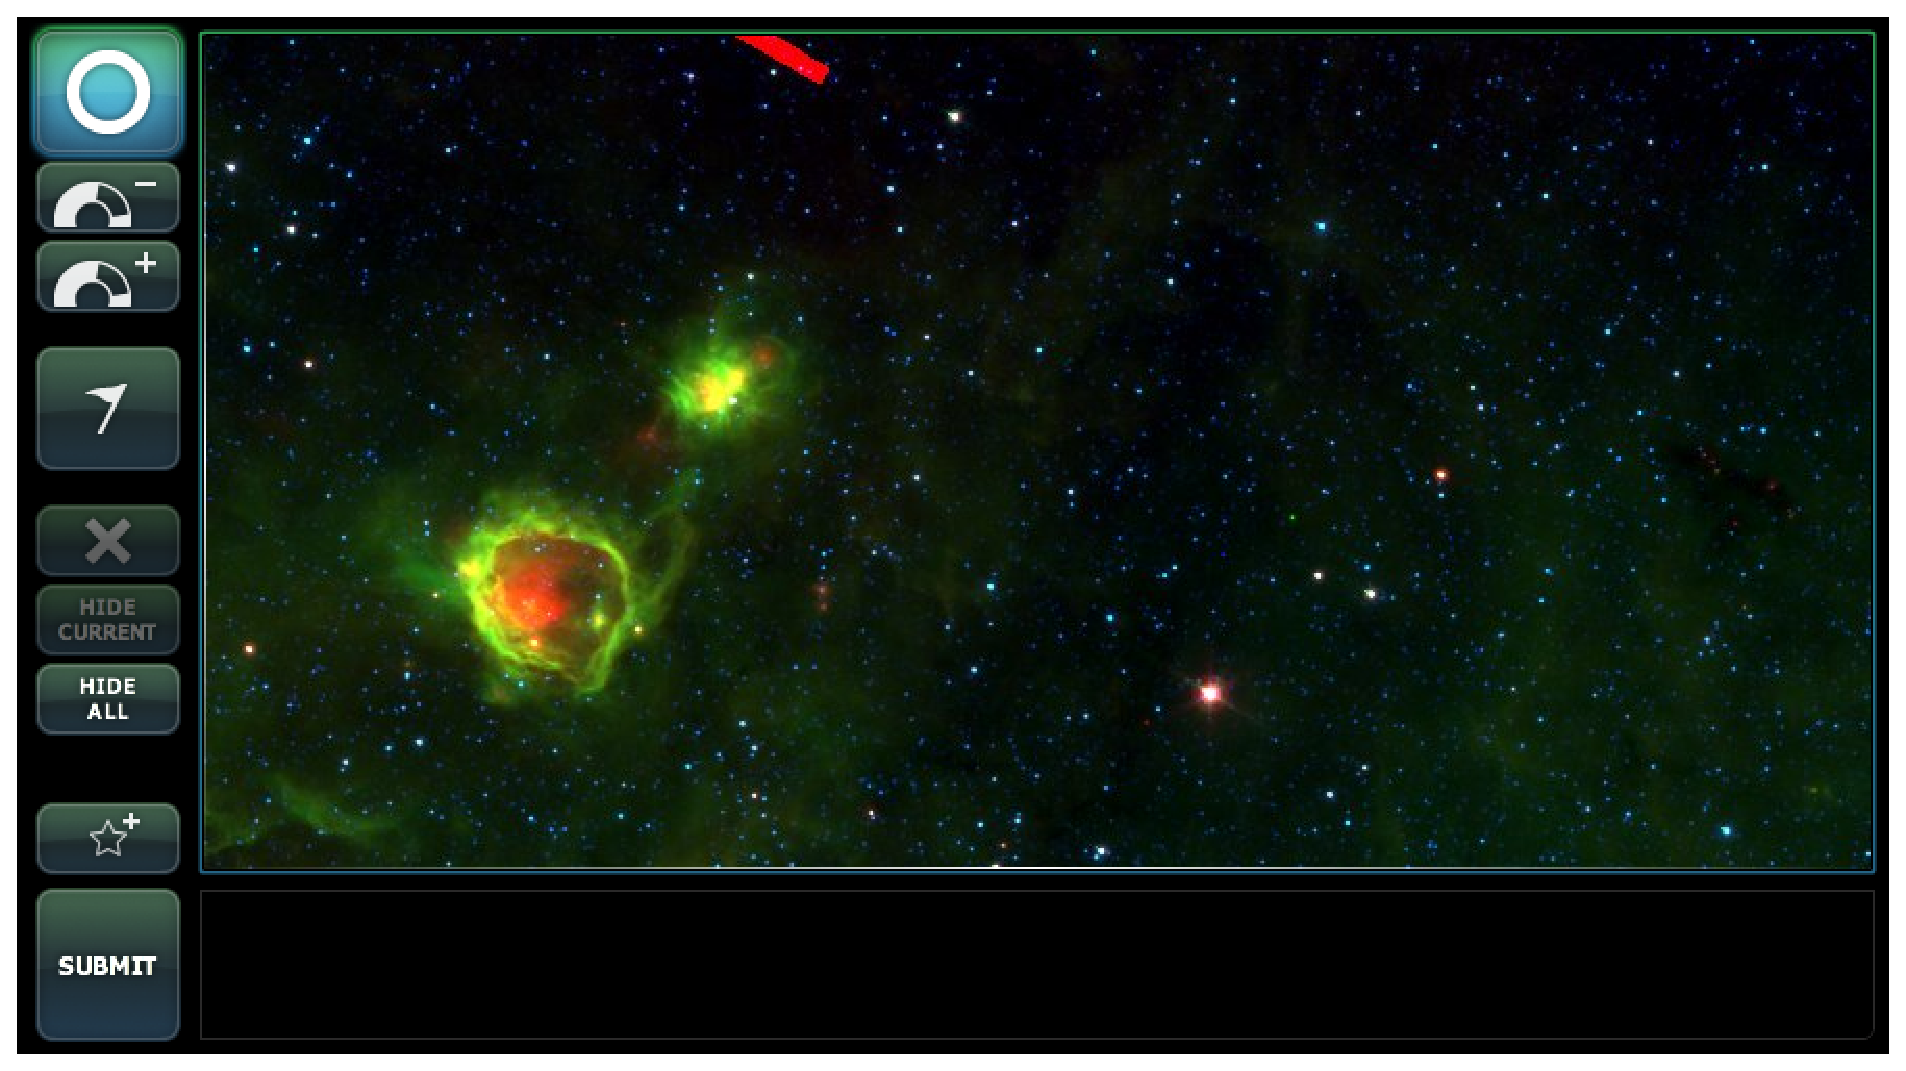
\includegraphics[width=0.48\textwidth]{./figures/user-interface.eps}
\caption{Screenshot of the Milky Way Project user interface. Colour figure available online.}
\label{user-interface}
\end{figure}

The assets in the MWP are multiband, false-colour JPEG images, created by gridding the {\it Spitzer} GLIMPSE and MIPSGAL mosaics into smaller images at three different zoom levels. The highest zoom level provides users with tiles of 0.3$^{\circ}\times$0.15$^{\circ}$, and at a resolution of 800$\times$400 pixels these tiles nearly reproduce the $1.2''$ pixel scale of the GLIMPSE survey images. Larger tile sizes of 0.75$^{\circ}\times$0.375$^{\circ}$ and 1.5$^{\circ}\times$0.75$^{\circ}$ were also generated. The tiles were plotted in an overlapping grid to allow all parts of the inner Galactic plane ($|l|\le 65\degree$, $|b|\le 1\degree$) to be viewed by the MWP users, at all zoom levels. To provide an optimal representation of the dynamic range within each tile, each of 3 single-band images was independently scaled to a square-root stretch function (with the faintest 5\% of image pixels clipped to black and the brightest 0.2\% clipped to white), assigned to a colour channel (red=24~\um, green=8.0~\um, blue=4.5~\um), and finally composited into a 3--colour image. The MIPSGAL 24~\um\ mosaics frequently saturate in regions of bright nebulosity, and saturated 24~\um\ pixels were set to maximum red to preserve the visual appeal of the images and to avoid presenting MWP users with saturation artefacts. The resulting composite images allow visual identification of both bright and faint features within a given image tile.

The MWP user interface (see Figure~\ref{user-interface}) was built using Flash, based upon the pre-existing Moon Zoo interface \citep{Joy+11}. Volunteers are primarily encouraged to draw ellipses onto the image to mark the locations of bubbles. A short, online tutorial shows how to use the tool, and examples of prominent bubbles are given\footnote{http://www.milkywayproject.org/tutorial}. As a secondary task, users can also mark rectangular areas of interest, which can be labelled as small bubbles, green knots, dark nebulae, star clusters, galaxies, fuzzy red objects or `other'. Examples of these are also given in a tutorial on the website, and these are discussed further in Section~\ref{other-objects}. Users can add as many annotations as they wish before submitting the image, at which point they are given another image for annotation. Each image's annotations are stored in a database as a classification, and users can see the images they have classified in a part of the site called `My Galaxy'. Users can only classify a given image once.

Volunteers are primarily asked to draw bubbles on the images, by placing elliptical annuli that match the structures they see in the data. They are also encouraged to mark other regions interest on an image, marking these are either star clusters, green knots, etc. Do do so, volunteers simply draw rectangles. Since these objects are secondary to the main bubble-finding task, the site was designed so that they should be simple and quick to mark. Simple rectangles allow us to record the positions and approximate sizes of any these other interesting objects.

\section{Catalogue construction}

\subsection{Galaxy images}

\begin{figure*}
\begin{center}
\subfigure[Candidate 1]{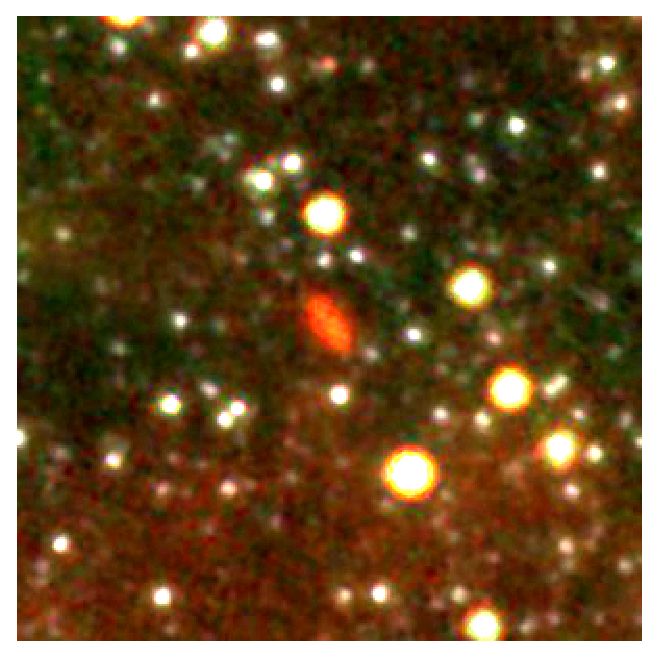
\includegraphics[width=0.19\textwidth]{./figures/3col/1.eps}}
\subfigure[Candidate 2]{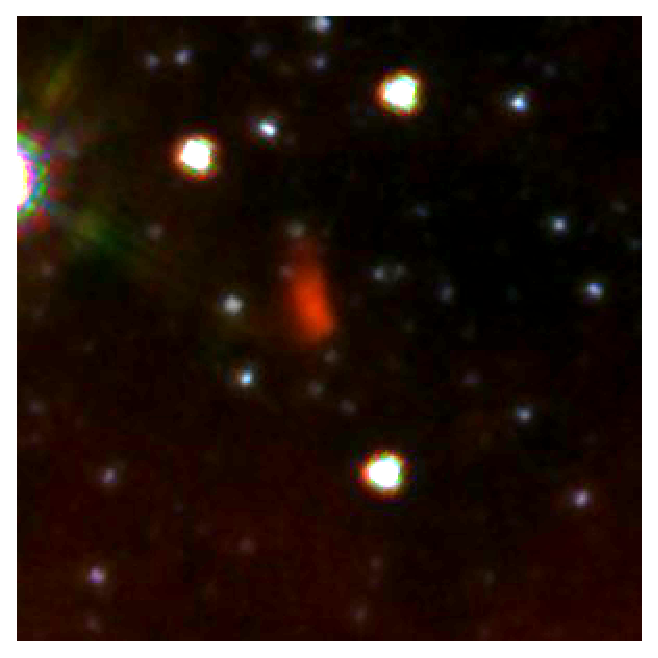
\includegraphics[width=0.19\textwidth]{./figures/3col/2.eps}}
\subfigure[Candidate 3]{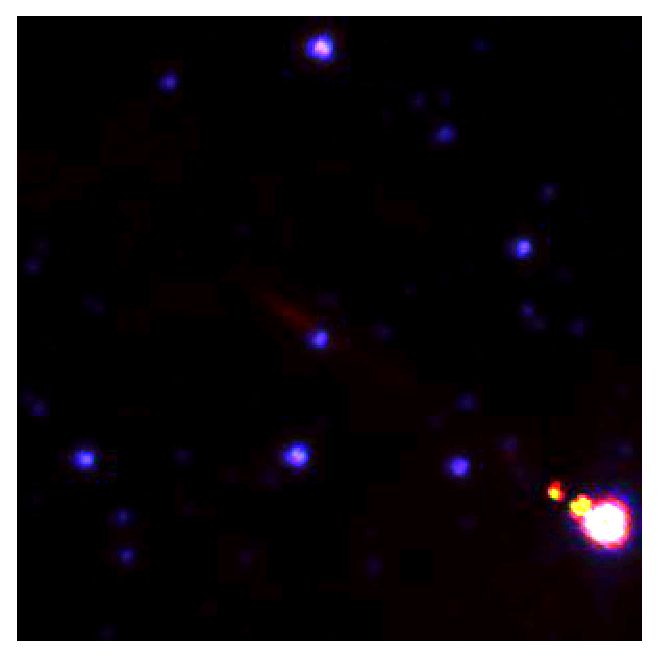
\includegraphics[width=0.19\textwidth]{./figures/3col/3.eps}}
\subfigure[Candidate 4]{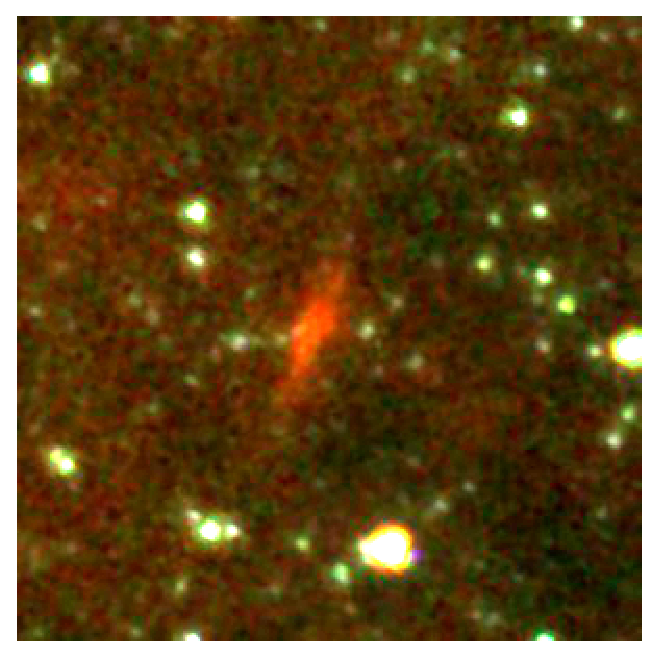
\includegraphics[width=0.19\textwidth]{./figures/3col/4.eps}}
\subfigure[Candidate 5]{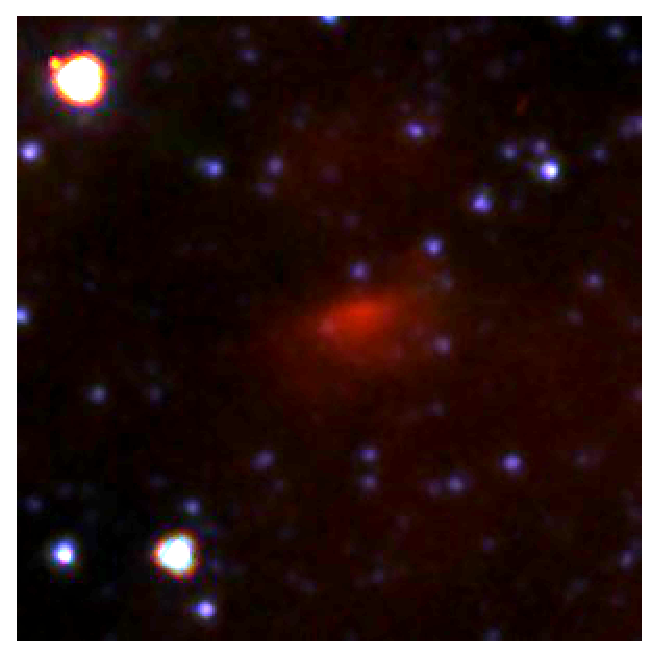
\includegraphics[width=0.19\textwidth]{./figures/3col/5.eps}}
\subfigure[Candidate 6]{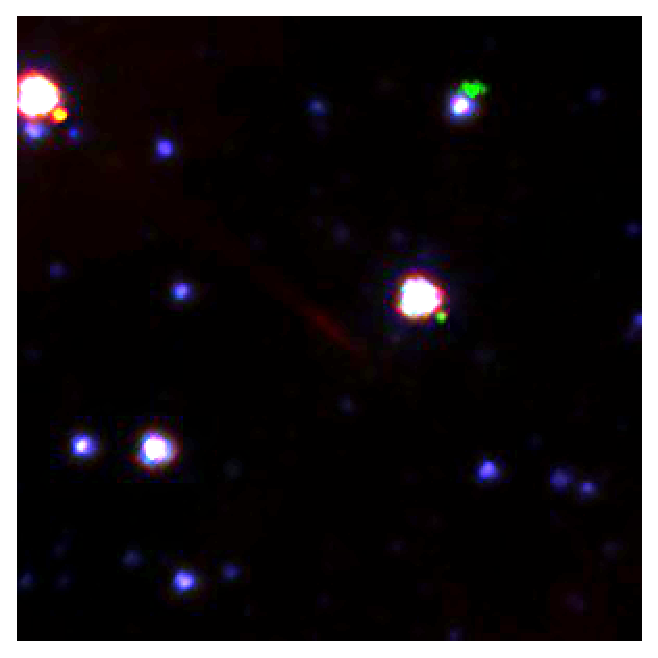
\includegraphics[width=0.19\textwidth]{./figures/3col/6.eps}}
\subfigure[Candidate 7]{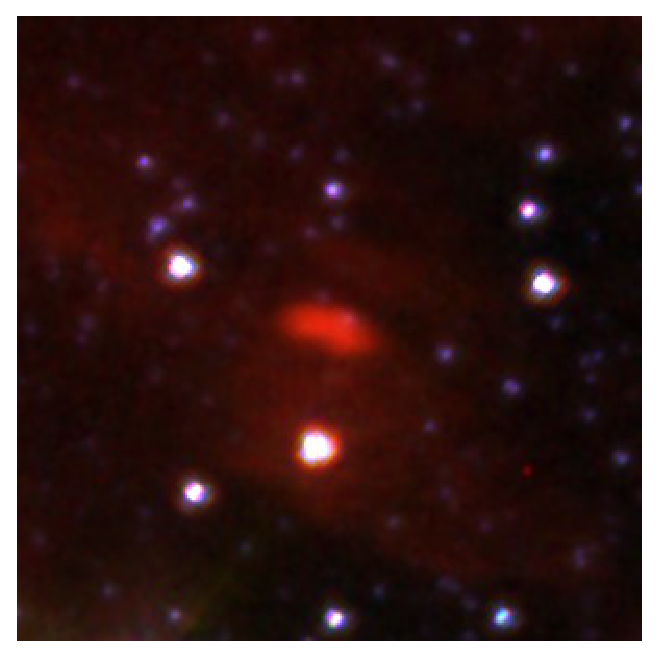
\includegraphics[width=0.19\textwidth]{./figures/3col/7.eps}}
\subfigure[Candidate 8]{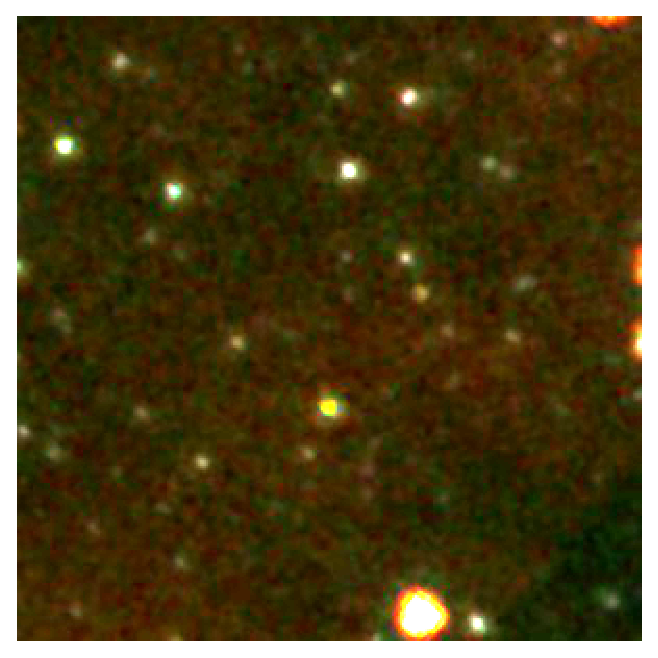
\includegraphics[width=0.19\textwidth]{./figures/3col/8.eps}}
\subfigure[Candidate 9]{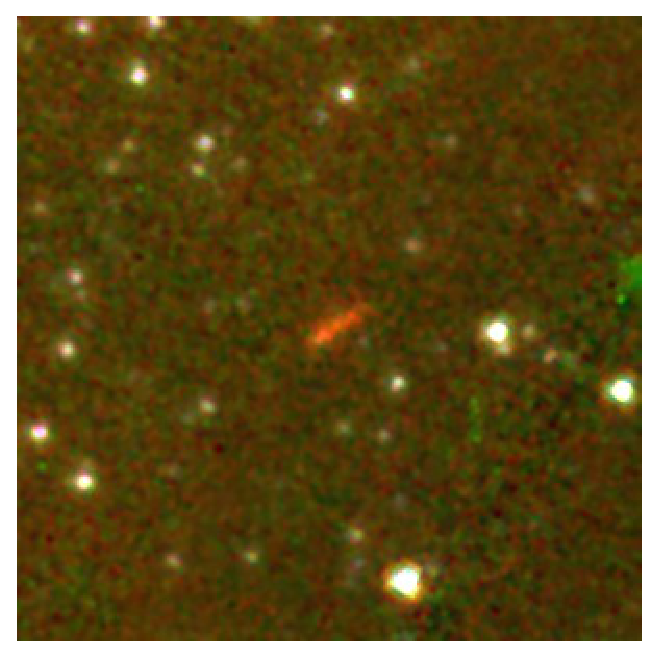
\includegraphics[width=0.19\textwidth]{./figures/3col/9.eps}}
\subfigure[Candidate 10]{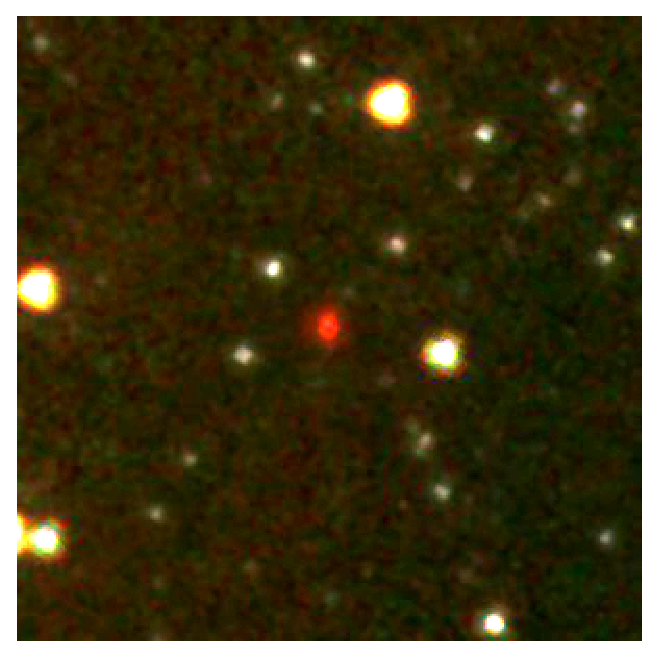
\includegraphics[width=0.19\textwidth]{./figures/3col/10.eps}}
\subfigure[Candidate 11]{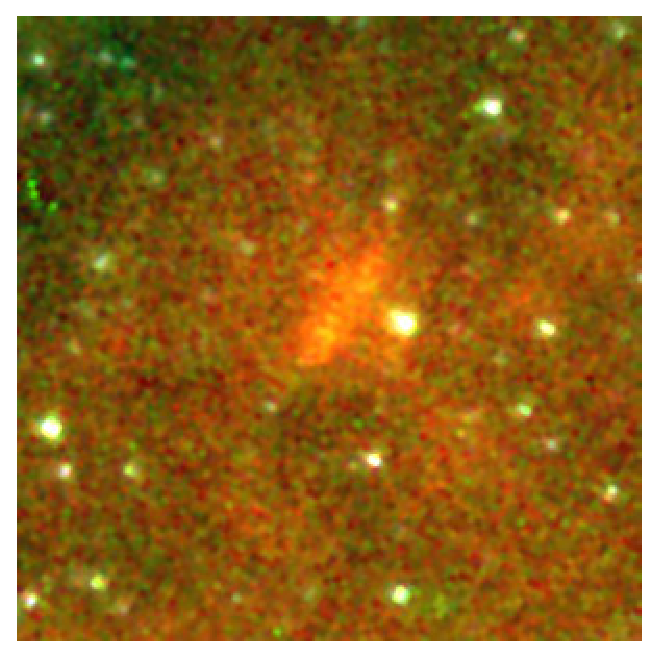
\includegraphics[width=0.19\textwidth]{./figures/3col/11.eps}}
\subfigure[Candidate 12]{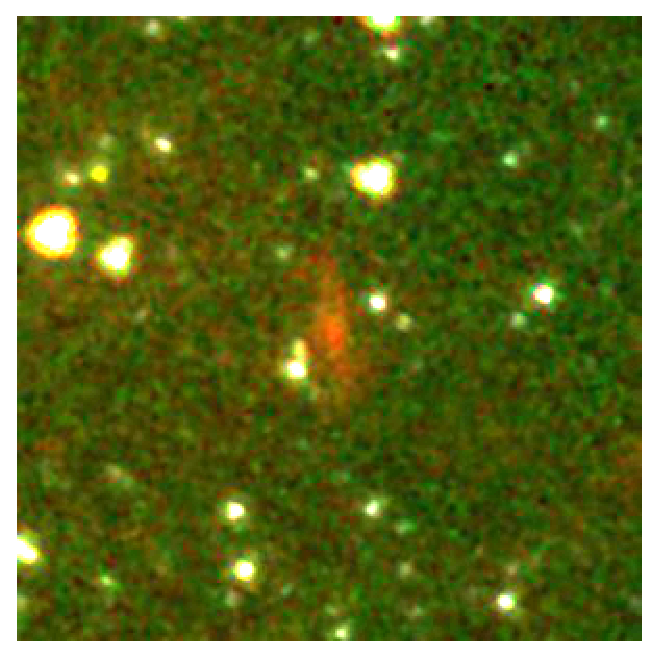
\includegraphics[width=0.19\textwidth]{./figures/3col/12.eps}}
\subfigure[Candidate 13]{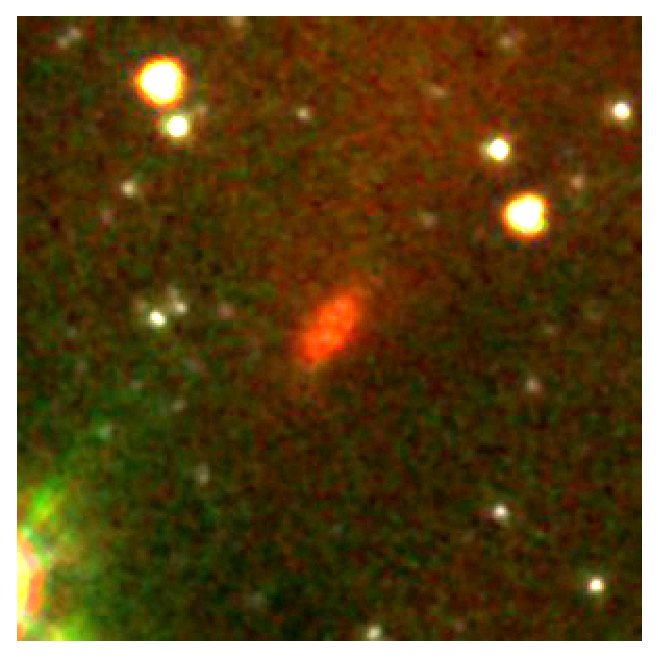
\includegraphics[width=0.19\textwidth]{./figures/3col/13.eps}}
\subfigure[Candidate 14]{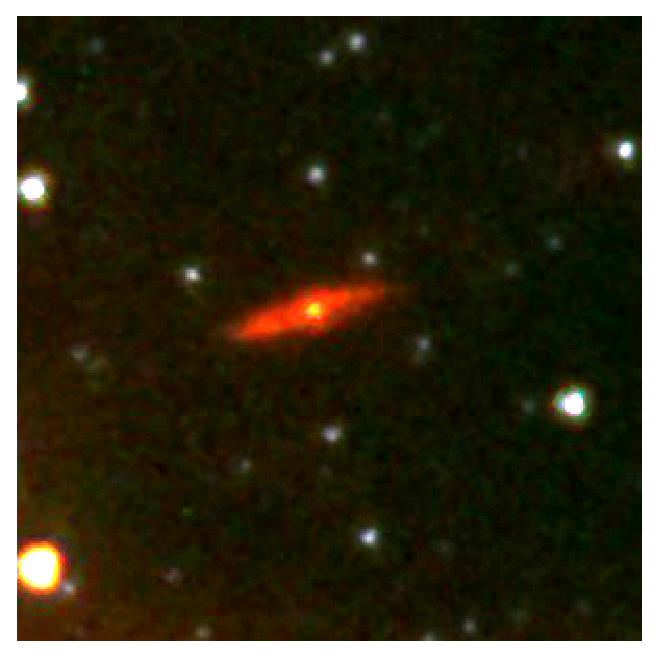
\includegraphics[width=0.19\textwidth]{./figures/3col/14.eps}}
\subfigure[Candidate 15]{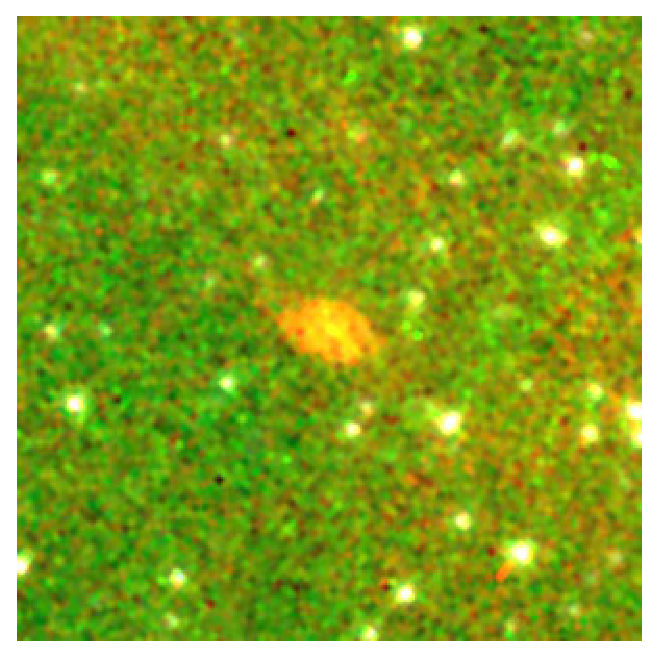
\includegraphics[width=0.19\textwidth]{./figures/3col/15.eps}}
\subfigure[Candidate 16]{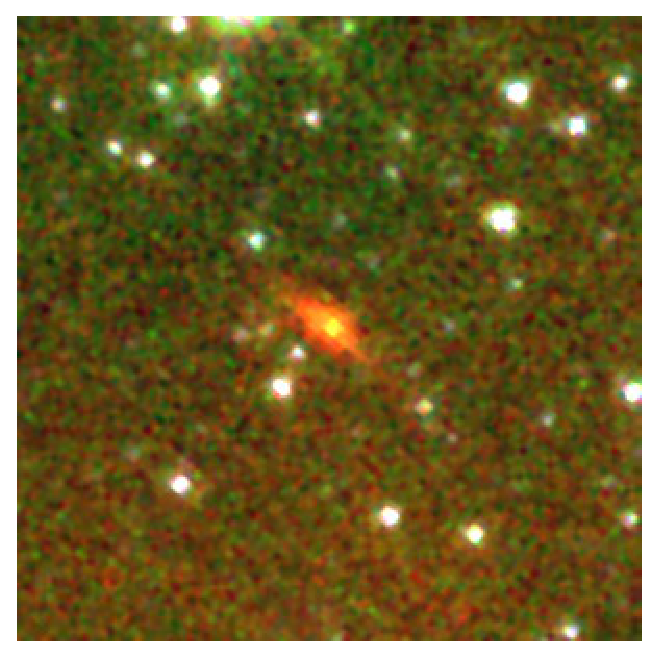
\includegraphics[width=0.19\textwidth]{./figures/3col/16.eps}}
\subfigure[Candidate 17]{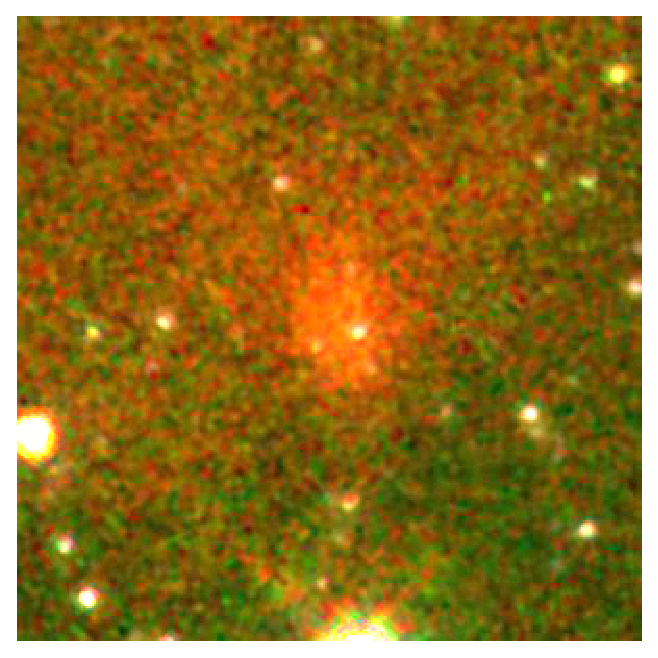
\includegraphics[width=0.19\textwidth]{./figures/3col/17.eps}}
\subfigure[Candidate 18]{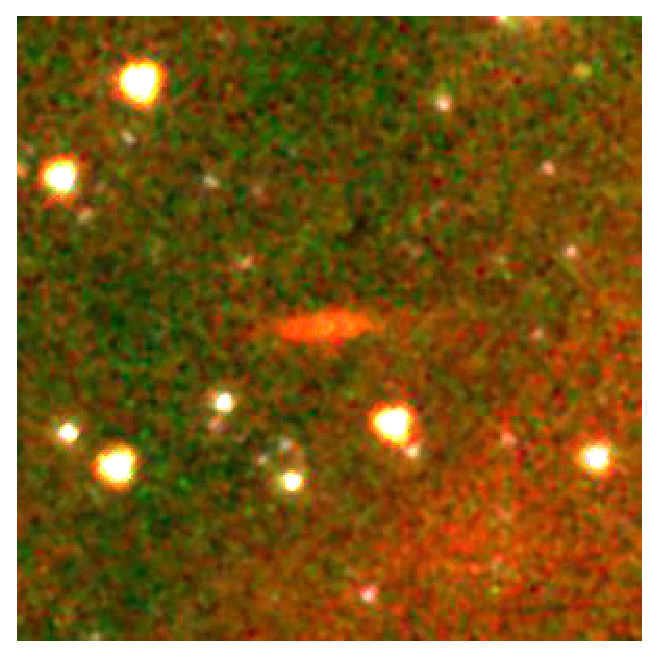
\includegraphics[width=0.19\textwidth]{./figures/3col/18.eps}}
\subfigure[Candidate 19]{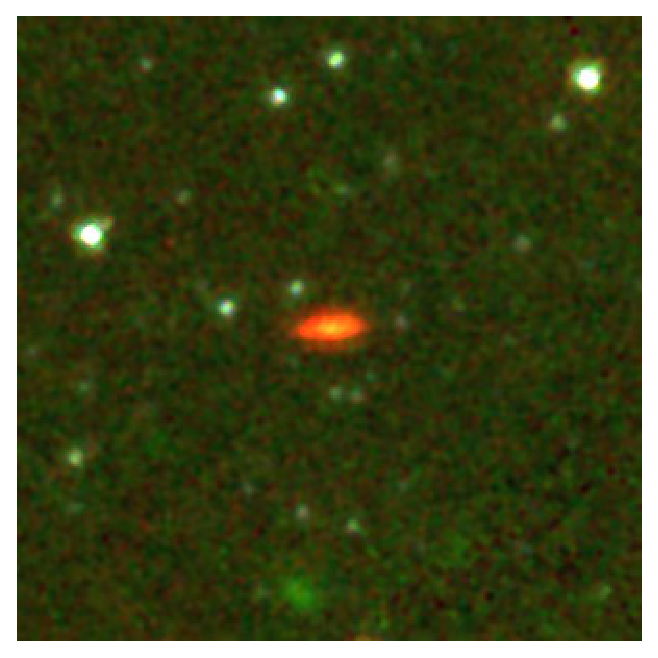
\includegraphics[width=0.19\textwidth]{./figures/3col/19.eps}}
\subfigure[Candidate 20]{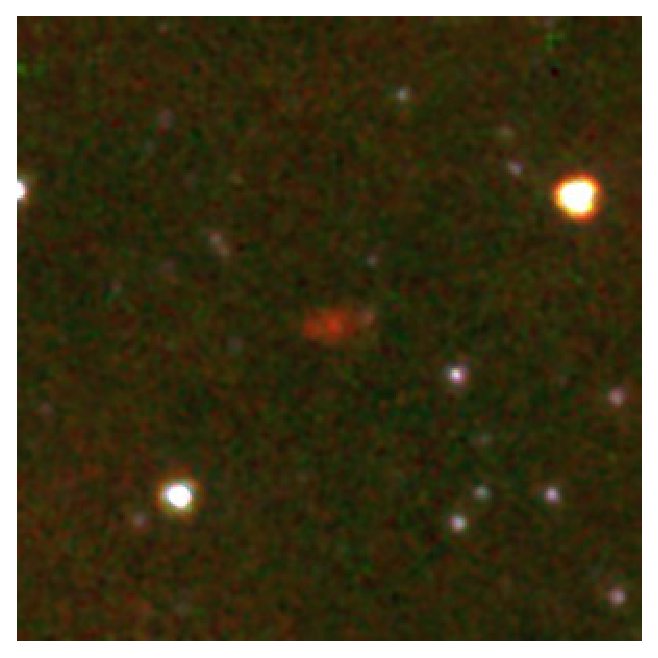
\includegraphics[width=0.19\textwidth]{./figures/3col/20.eps}}
\subfigure[Candidate 21]{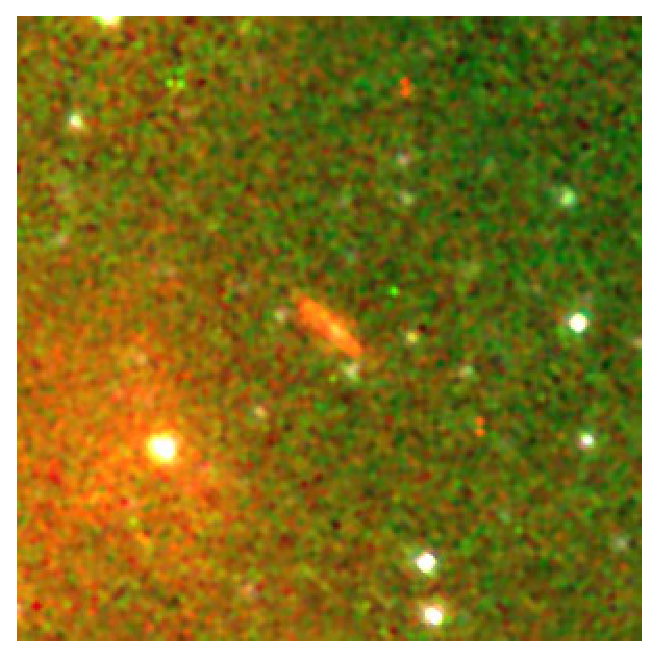
\includegraphics[width=0.19\textwidth]{./figures/3col/21.eps}}
\subfigure[Candidate 22]{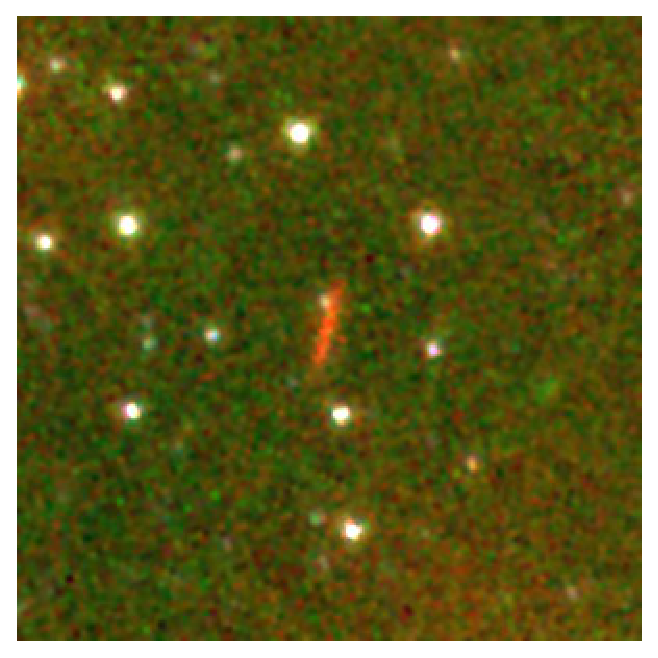
\includegraphics[width=0.19\textwidth]{./figures/3col/22.eps}}
\subfigure[Candidate 23]{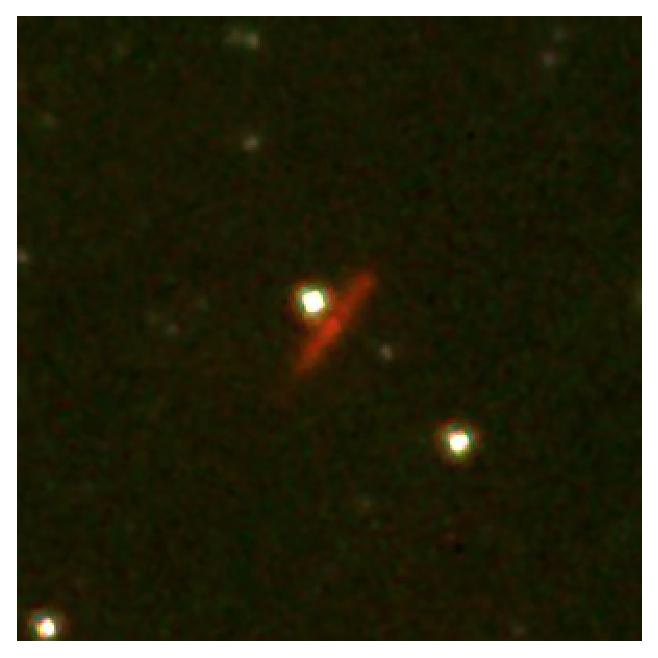
\includegraphics[width=0.19\textwidth]{./figures/3col/23.eps}}
\subfigure[Candidate 24]{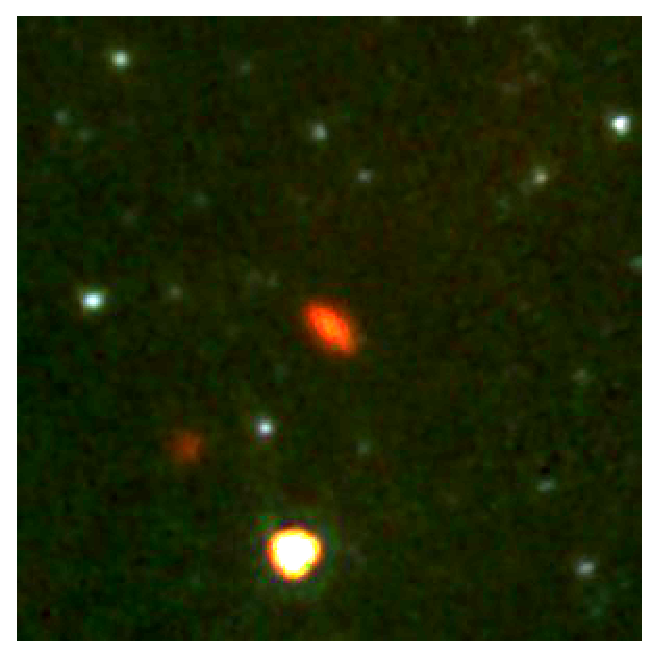
\includegraphics[width=0.19\textwidth]{./figures/3col/24.eps}}
\subfigure[Candidate 25]{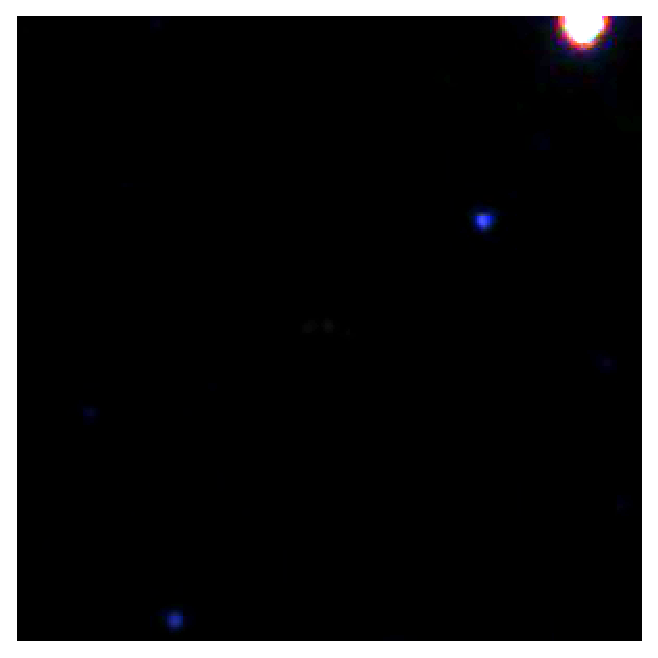
\includegraphics[width=0.19\textwidth]{./figures/3col/25.eps}}
\caption{Three-colour composite images of candidate galaxies 1--25, with RGB channels using Spitzer IRAC bands 8$\mu$m, 4.5$\mu$m and 3.6$\mu$m respectively.}
\label{gal1}
\end{center}
\end{figure*} 

\begin{figure*}
\begin{center}
\subfigure[Candidate 26]{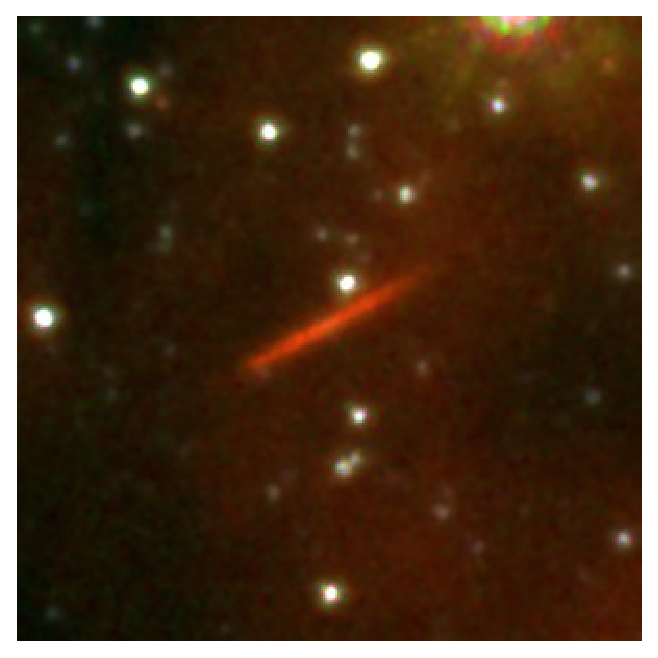
\includegraphics[width=0.19\textwidth]{./figures/3col/26.eps}}
\subfigure[Candidate 27]{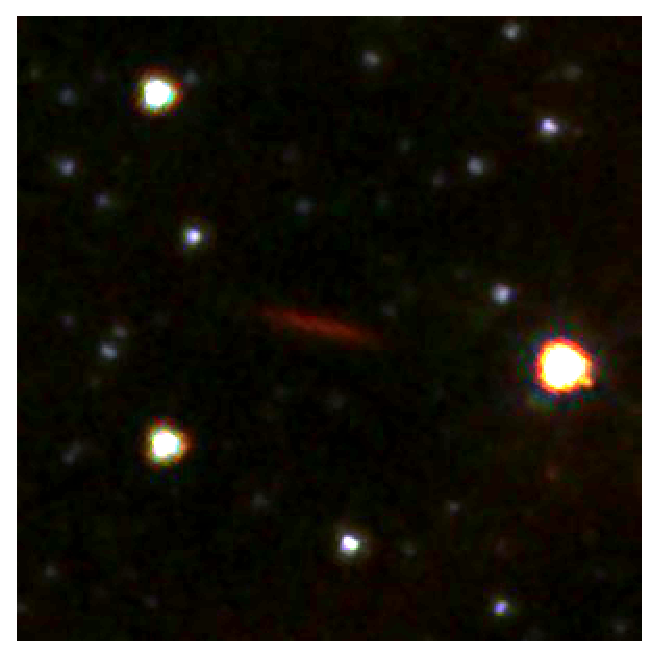
\includegraphics[width=0.19\textwidth]{./figures/3col/27.eps}}
\subfigure[Candidate 28]{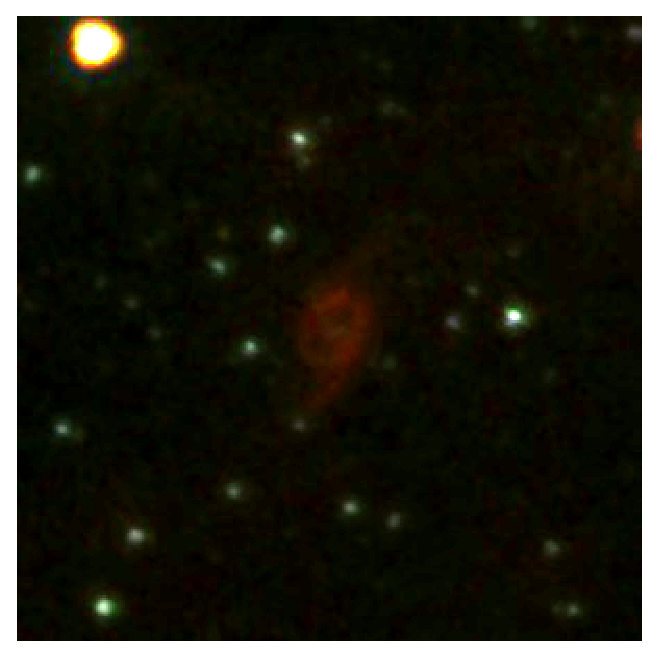
\includegraphics[width=0.19\textwidth]{./figures/3col/28.eps}}
\subfigure[Candidate 29]{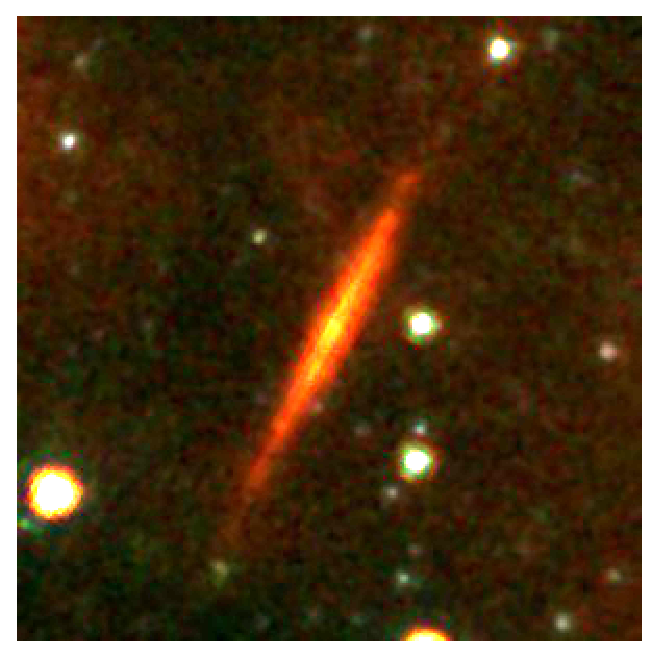
\includegraphics[width=0.19\textwidth]{./figures/3col/29.eps}}
\subfigure[Candidate 30]{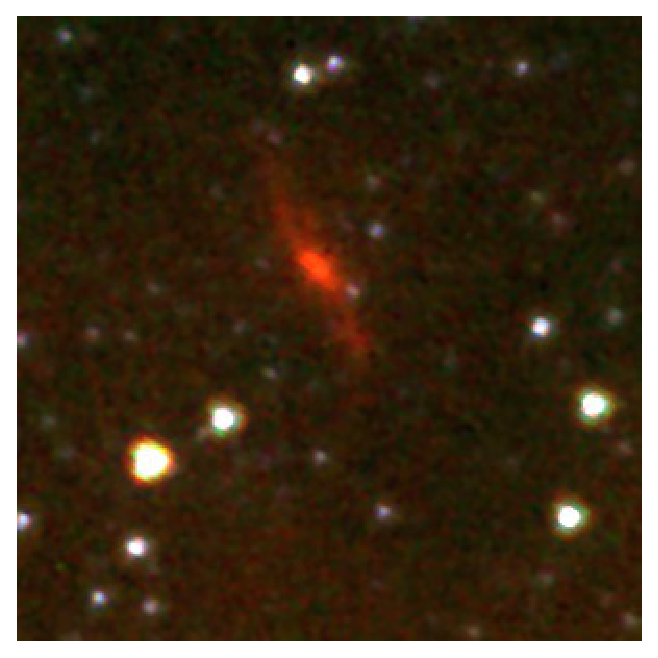
\includegraphics[width=0.19\textwidth]{./figures/3col/30.eps}}
\subfigure[Candidate 31]{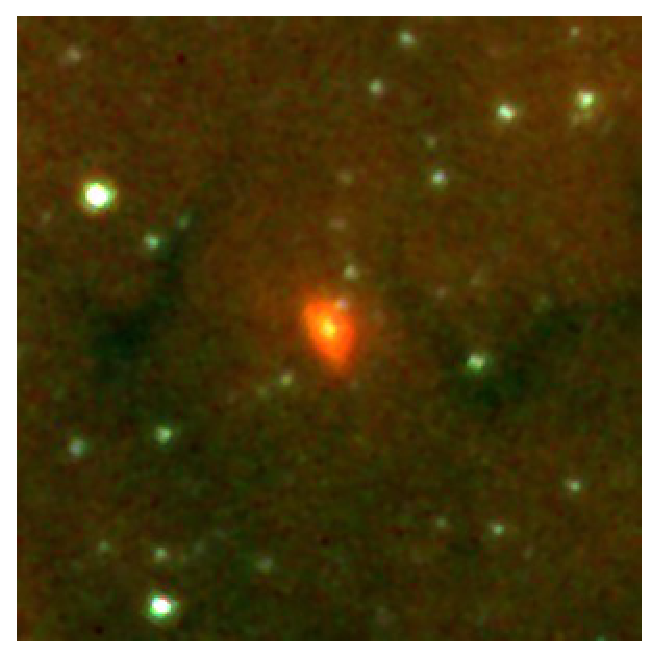
\includegraphics[width=0.19\textwidth]{./figures/3col/31.eps}}
\subfigure[Candidate 32]{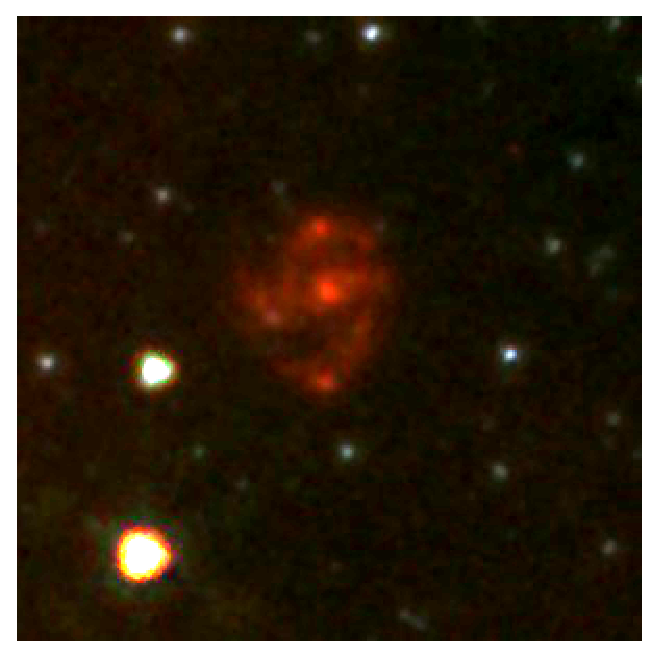
\includegraphics[width=0.19\textwidth]{./figures/3col/32.eps}}
\subfigure[Candidate 33]{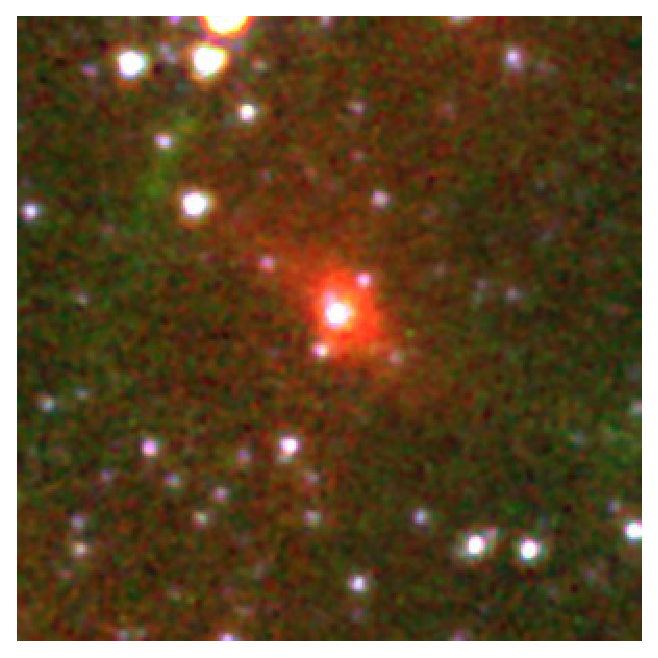
\includegraphics[width=0.19\textwidth]{./figures/3col/33.eps}}
\subfigure[Candidate 34]{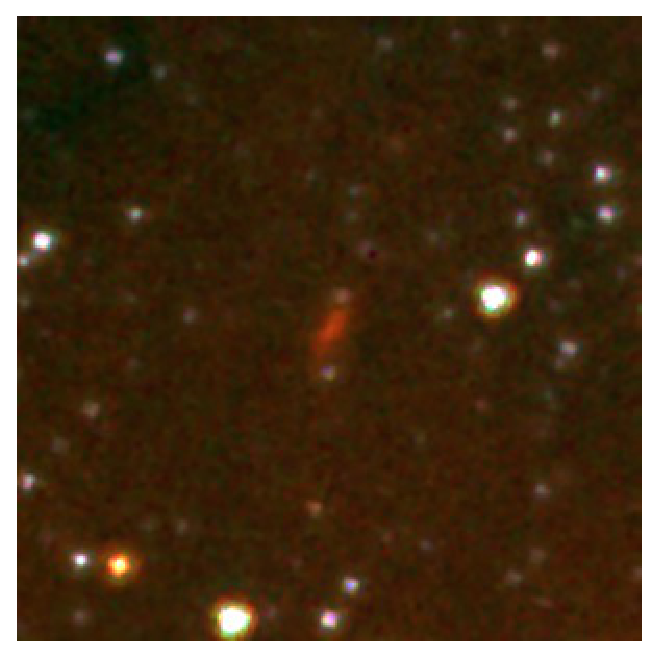
\includegraphics[width=0.19\textwidth]{./figures/3col/34.eps}}
\subfigure[Candidate 35]{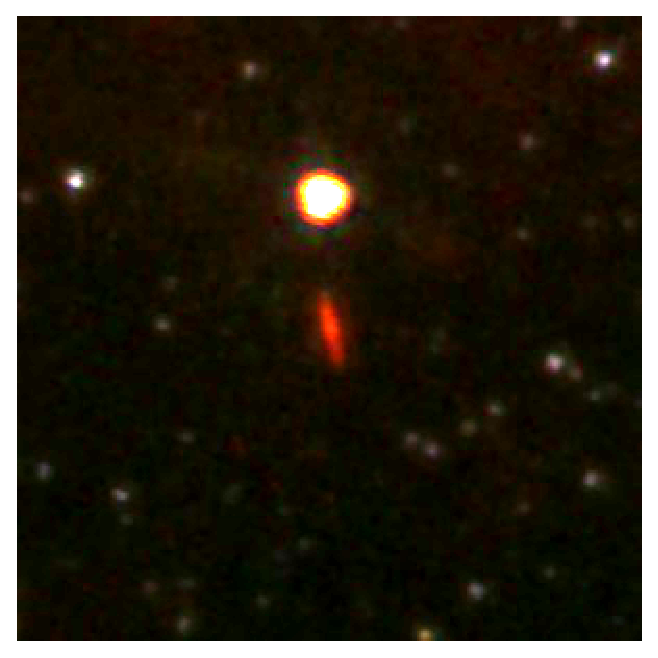
\includegraphics[width=0.19\textwidth]{./figures/3col/35.eps}}
\subfigure[Candidate 36]{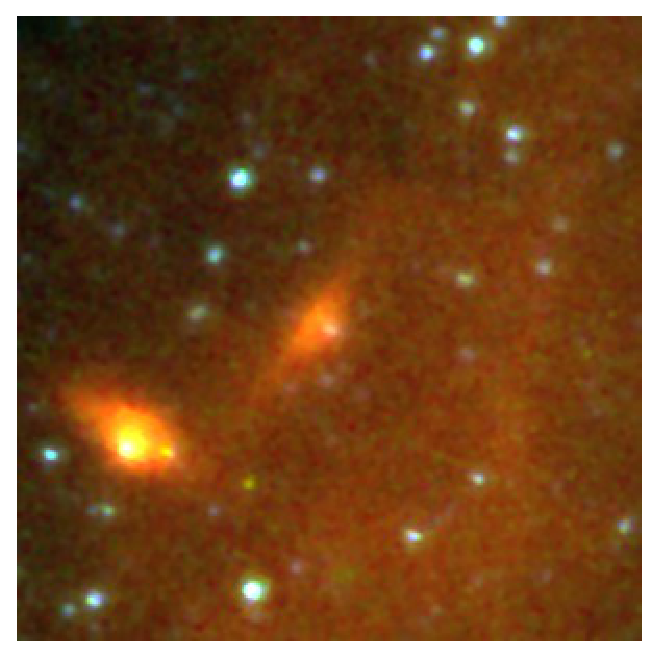
\includegraphics[width=0.19\textwidth]{./figures/3col/36.eps}}
\subfigure[Candidate 37]{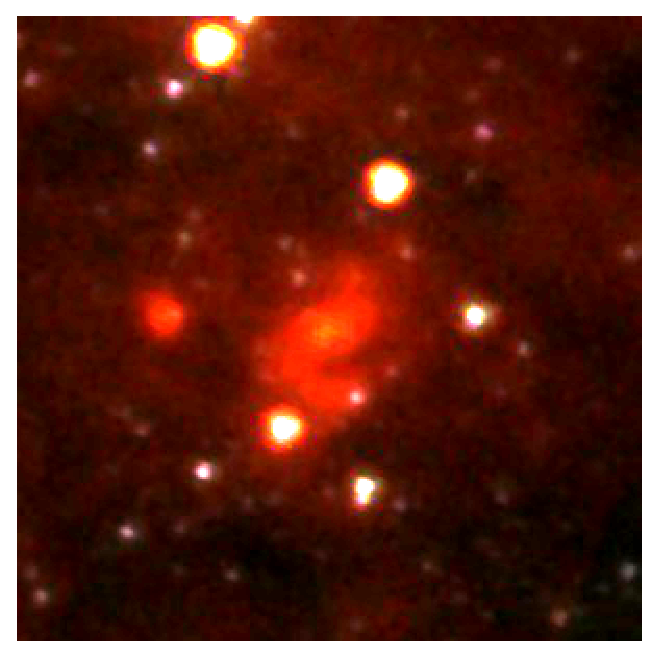
\includegraphics[width=0.19\textwidth]{./figures/3col/37.eps}}
\subfigure[Candidate 38]{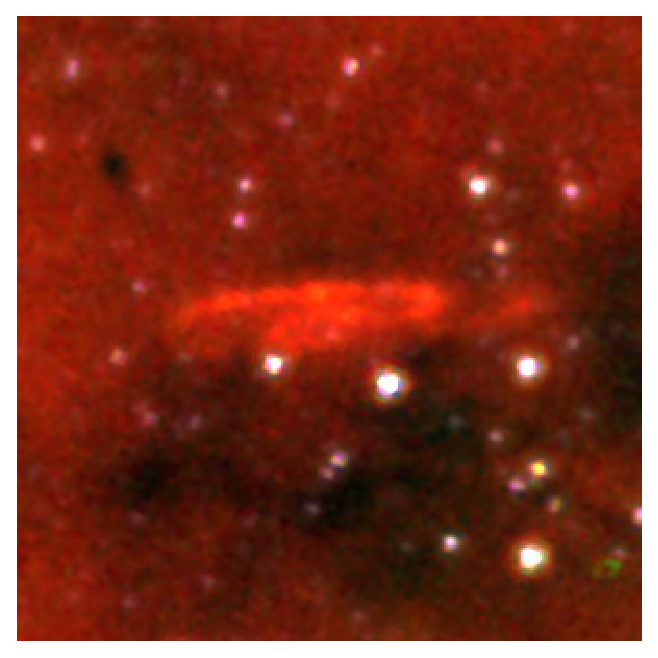
\includegraphics[width=0.19\textwidth]{./figures/3col/38.eps}}
\subfigure[Candidate 39]{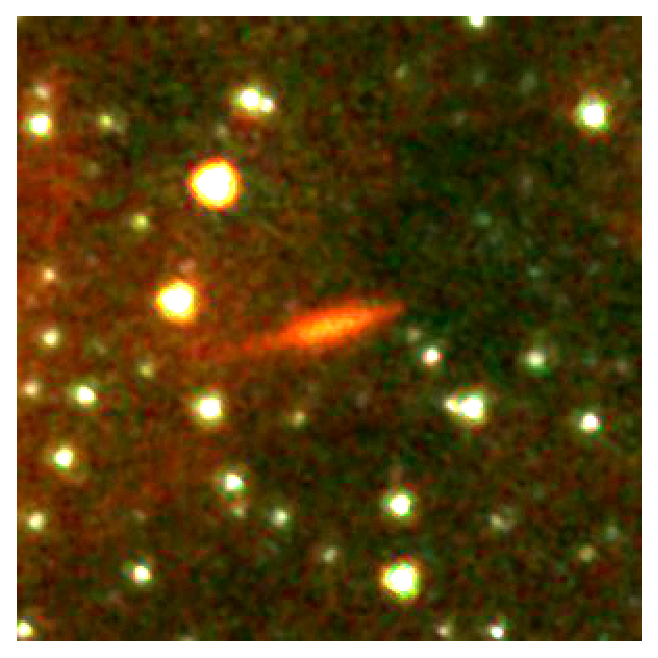
\includegraphics[width=0.19\textwidth]{./figures/3col/39.eps}}
\subfigure[Candidate 40]{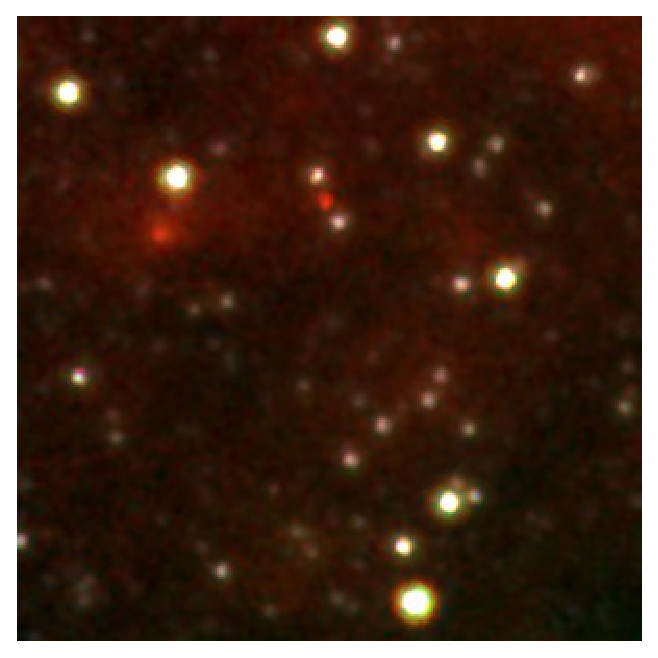
\includegraphics[width=0.19\textwidth]{./figures/3col/40.eps}}
\subfigure[Candidate 41]{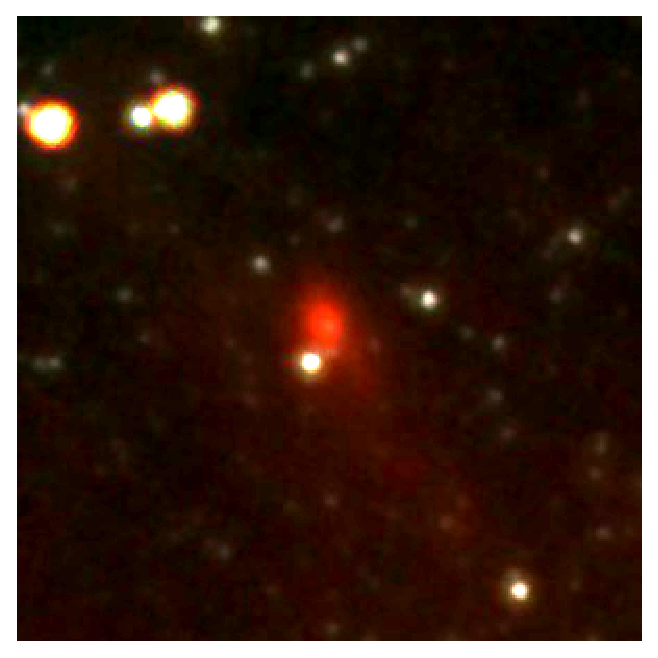
\includegraphics[width=0.19\textwidth]{./figures/3col/41.eps}}
\subfigure[Candidate 42]{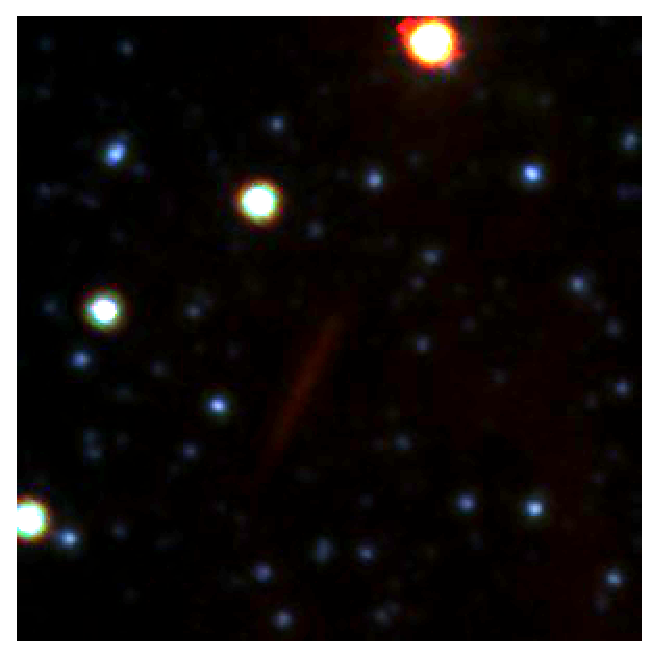
\includegraphics[width=0.19\textwidth]{./figures/3col/42.eps}}
\subfigure[Candidate 43]{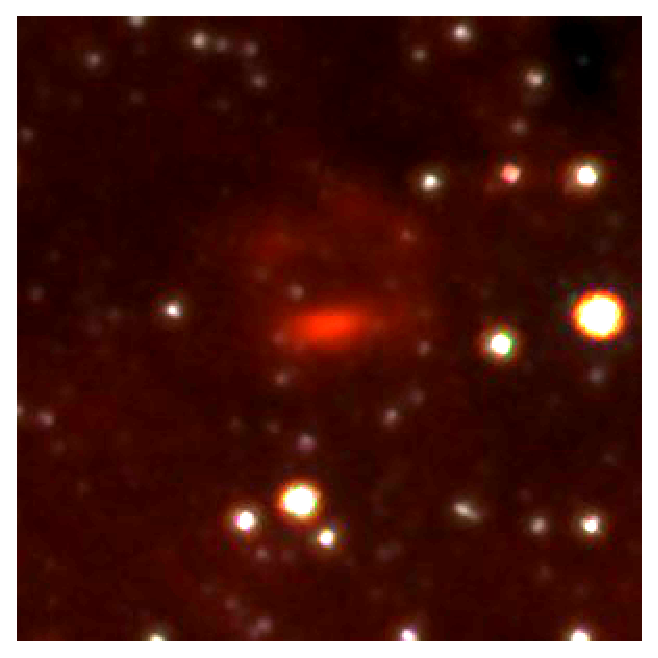
\includegraphics[width=0.19\textwidth]{./figures/3col/43.eps}}
\caption{Three-colour composite images of candidate galaxies 26--43, with RGB channels using Spitzer IRAC bands 8$\mu$m, 4.5$\mu$m and 3.6$\mu$m respectively.}
\label{gal1}
\end{center}
\end{figure*} 

\subsection{Aperture photometry}

\subsection{Galaxy catalogue}

\section{Results}

\subsection{Spectral energy distributions}

\subsection{Comparison with large-scale structure from 2MASS}

\section{Discussion}

\section{Summary and future work}

\section*{Acknowledgments}

This publication has been made possible by the participation of more than 40,000 volunteers on the Milky Way Project. Their contributions are acknowledged individually at http://www.milkywayproject.org/authors.

The Milky Way Project, and R.J.S. were supported by The Leverhulme Trust. The `Talk' discussion tool used in the MWP was developed at the Adler Planetarium with support from the National Science Foundation CDI grant : DRL-0941610. 

This work is based on observations made with the Spitzer Space Telescope, which is operated by the Jet Propulsion Laboratory, California Institute of Technology under a contract with NASA.

\bibliographystyle{apj}
\bibliography{mwpref}

\clearpage

\appendix{Galaxy Images and SEDs}

\begin{figure*}
\begin{center}
\subfigure[]{
\includegraphics[width=0.22\textwidth]{./figures/cutouts/1.jpg.eps}}
\subfigure[]{
\includegraphics[width=0.22\textwidth]{./figures/IRAC4/1.jpg.eps}}
\subfigure[]{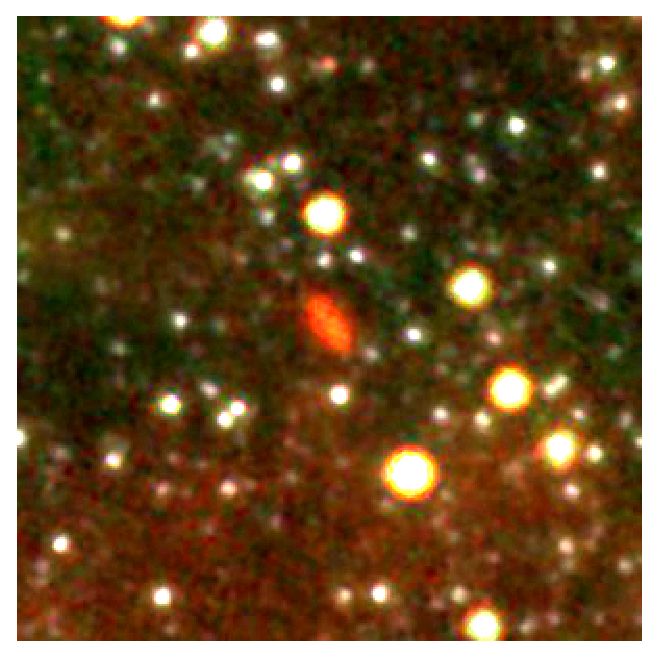
\includegraphics[width=0.22\textwidth]{./figures/3col/1.eps}}
\subfigure[]{\includegraphics[width=0.32\textwidth]{./figures/seds/gal1.eps}}
\caption{Data for galaxy candidate 1. Subfigures show (a) MWP image cutout; (b) IRAC 8$\mu$m data; (c) Three-colour composite with RGB channels using Spitzer IRAC bands 8$\mu$m, 4.5$\mu$m and 3.6$\mu$m respectively; and (d) measured SED for this object.}
\label{gal1}
\end{center}
\end{figure*} 

\begin{figure*}
\begin{center}
\subfigure[]{
\includegraphics[width=0.22\textwidth]{./figures/cutouts/2.jpg.eps}}
\subfigure[]{
\includegraphics[width=0.22\textwidth]{./figures/IRAC4/2.jpg.eps}}
\subfigure[]{\includegraphics[width=0.22\textwidth]{./figures/3col/2.eps}}
\subfigure[]{\includegraphics[width=0.32\textwidth]{./figures/seds/gal2.eps}}
\caption{Data for galaxy candidate 2. Subfigures show (a) MWP image cutout; (b) IRAC 8$\mu$m data; (c) Three-colour composite with RGB channels using Spitzer IRAC bands 8$\mu$m, 4.5$\mu$m and 3.6$\mu$m respectively; and (d) measured SED for this object.}
\label{gal1}
\end{center}
\end{figure*} 

\begin{figure*}
\begin{center}
\subfigure[]{\includegraphics[width=0.22\textwidth]{./figures/cutouts/3.jpg.eps}}
\subfigure[]{\includegraphics[width=0.22\textwidth]{./figures/IRAC4/3.jpg.eps}}
\subfigure[]{\includegraphics[width=0.22\textwidth]{./figures/3col/3.eps}}
\subfigure[]{\includegraphics[width=0.32\textwidth]{./figures/seds/gal3.eps}}
\caption{Data for galaxy candidate 3. Subfigures show (a) MWP image cutout; (b) IRAC 8$\mu$m data; (c) Three-colour composite with RGB channels using Spitzer IRAC bands 8$\mu$m, 4.5$\mu$m and 3.6$\mu$m respectively; and (d) measured SED for this object.}
\label{gal1}
\end{center}
\end{figure*} 

\begin{figure*}
\begin{center}
\subfigure[]{\includegraphics[width=0.22\textwidth]{./figures/cutouts/4.jpg.eps}}
\subfigure[]{\includegraphics[width=0.22\textwidth]{./figures/IRAC4/4.jpg.eps}}
\subfigure[]{\includegraphics[width=0.22\textwidth]{./figures/3col/4.eps}}
\subfigure[]{\includegraphics[width=0.32\textwidth]{./figures/seds/gal4.eps}}
\caption{Data for galaxy candidate 4. Subfigures show (a) MWP image cutout; (b) IRAC 8$\mu$m data; (c) Three-colour composite with RGB channels using Spitzer IRAC bands 8$\mu$m, 4.5$\mu$m and 3.6$\mu$m respectively; and (d) measured SED for this object.}
\label{gal1}
\end{center}
\end{figure*} 

\begin{figure*}
\begin{center}
\subfigure[]{\includegraphics[width=0.22\textwidth]{./figures/cutouts/5.jpg.eps}}
\subfigure[]{\includegraphics[width=0.22\textwidth]{./figures/IRAC4/5.jpg.eps}}
\subfigure[]{\includegraphics[width=0.22\textwidth]{./figures/3col/5.eps}}
\subfigure[]{\includegraphics[width=0.32\textwidth]{./figures/seds/gal5.eps}}
\caption{Data for galaxy candidate 5. Subfigures show (a) MWP image cutout; (b) IRAC 8$\mu$m data; (c) Three-colour composite with RGB channels using Spitzer IRAC bands 8$\mu$m, 4.5$\mu$m and 3.6$\mu$m respectively; and (d) measured SED for this object.}
\label{gal1}
\end{center}
\end{figure*} 




\begin{figure*}
\begin{center}
\subfigure[]{\includegraphics[width=0.22\textwidth]{./figures/cutouts/7.jpg.eps}}
\subfigure[]{\includegraphics[width=0.22\textwidth]{./figures/IRAC4/7.jpg.eps}}
\subfigure[]{\includegraphics[width=0.22\textwidth]{./figures/3col/7.eps}}
\subfigure[]{\includegraphics[width=0.32\textwidth]{./figures/seds/gal7.eps}}
\caption{Data for galaxy candidate 7. Subfigures show (a) MWP image cutout; (b) IRAC 8$\mu$m data; (c) Three-colour composite with RGB channels using Spitzer IRAC bands 8$\mu$m, 4.5$\mu$m and 3.6$\mu$m respectively; and (d) measured SED for this object.}
\label{gal1}
\end{center}
\end{figure*} 

\begin{figure*}
\begin{center}
\subfigure[]{\includegraphics[width=0.22\textwidth]{./figures/cutouts/8.jpg.eps}}
\subfigure[]{\includegraphics[width=0.22\textwidth]{./figures/IRAC4/8.jpg.eps}}
\subfigure[]{\includegraphics[width=0.22\textwidth]{./figures/3col/8.eps}}
\subfigure[]{\includegraphics[width=0.32\textwidth]{./figures/seds/gal8.eps}}
\caption{Data for galaxy candidate 8. Subfigures show (a) MWP image cutout; (b) IRAC 8$\mu$m data; (c) Three-colour composite with RGB channels using Spitzer IRAC bands 8$\mu$m, 4.5$\mu$m and 3.6$\mu$m respectively; and (d) measured SED for this object.}
\label{gal1}
\end{center}
\end{figure*} 

\begin{figure*}
\begin{center}
\subfigure[]{\includegraphics[width=0.22\textwidth]{./figures/cutouts/9.jpg.eps}}
\subfigure[]{\includegraphics[width=0.22\textwidth]{./figures/IRAC4/9.jpg.eps}}
\subfigure[]{\includegraphics[width=0.22\textwidth]{./figures/3col/9.eps}}
\subfigure[]{\includegraphics[width=0.32\textwidth]{./figures/seds/gal9.eps}}
\caption{Data for galaxy candidate 9. Subfigures show (a) MWP image cutout; (b) IRAC 8$\mu$m data; (c) Three-colour composite with RGB channels using Spitzer IRAC bands 8$\mu$m, 4.5$\mu$m and 3.6$\mu$m respectively; and (d) measured SED for this object.}
\label{gal1}
\end{center}
\end{figure*} 

\begin{figure*}
\begin{center}
\subfigure[]{\includegraphics[width=0.22\textwidth]{./figures/cutouts/10.jpg.eps}}
\subfigure[]{\includegraphics[width=0.22\textwidth]{./figures/IRAC4/10.jpg.eps}}
\subfigure[]{\includegraphics[width=0.22\textwidth]{./figures/3col/10.eps}}
\subfigure[]{\includegraphics[width=0.32\textwidth]{./figures/seds/gal10.eps}}
\caption{Data for galaxy candidate 10. Subfigures show (a) MWP image cutout; (b) IRAC 8$\mu$m data; (c) Three-colour composite with RGB channels using Spitzer IRAC bands 8$\mu$m, 4.5$\mu$m and 3.6$\mu$m respectively; and (d) measured SED for this object.}
\label{gal1}
\end{center}
\end{figure*} 

\begin{figure*}
\begin{center}
\subfigure[]{\includegraphics[width=0.22\textwidth]{./figures/cutouts/11.jpg.eps}}
\subfigure[]{\includegraphics[width=0.22\textwidth]{./figures/IRAC4/11.jpg.eps}}
\subfigure[]{\includegraphics[width=0.22\textwidth]{./figures/3col/11.eps}}
\subfigure[]{\includegraphics[width=0.32\textwidth]{./figures/seds/gal11.eps}}
\caption{Data for galaxy candidate 11. Subfigures show (a) MWP image cutout; (b) IRAC 8$\mu$m data; (c) Three-colour composite with RGB channels using Spitzer IRAC bands 8$\mu$m, 4.5$\mu$m and 3.6$\mu$m respectively; and (d) measured SED for this object.}
\label{gal1}
\end{center}
\end{figure*} 

\begin{figure*}
\begin{center}
\subfigure[]{\includegraphics[width=0.22\textwidth]{./figures/cutouts/12.jpg.eps}}
\subfigure[]{\includegraphics[width=0.22\textwidth]{./figures/IRAC4/12.jpg.eps}}
\subfigure[]{\includegraphics[width=0.22\textwidth]{./figures/3col/12.eps}}
\subfigure[]{\includegraphics[width=0.32\textwidth]{./figures/seds/gal12.eps}}
\caption{Data for galaxy candidate 12. Subfigures show (a) MWP image cutout; (b) IRAC 8$\mu$m data; (c) Three-colour composite with RGB channels using Spitzer IRAC bands 8$\mu$m, 4.5$\mu$m and 3.6$\mu$m respectively; and (d) measured SED for this object.}
\label{gal1}
\end{center}
\end{figure*} 

\begin{figure*}
\begin{center}
\subfigure[]{\includegraphics[width=0.22\textwidth]{./figures/cutouts/13.jpg.eps}}
\subfigure[]{\includegraphics[width=0.22\textwidth]{./figures/IRAC4/13.jpg.eps}}
\subfigure[]{\includegraphics[width=0.22\textwidth]{./figures/3col/13.eps}}
\subfigure[]{\includegraphics[width=0.32\textwidth]{./figures/seds/gal13.eps}}
\caption{Data for galaxy candidate 13. Subfigures show (a) MWP image cutout; (b) IRAC 8$\mu$m data; (c) Three-colour composite with RGB channels using Spitzer IRAC bands 8$\mu$m, 4.5$\mu$m and 3.6$\mu$m respectively; and (d) measured SED for this object.}
\label{gal1}
\end{center}
\end{figure*} 

\begin{figure*}
\begin{center}
\subfigure[]{\includegraphics[width=0.22\textwidth]{./figures/cutouts/14.jpg.eps}}
\subfigure[]{\includegraphics[width=0.22\textwidth]{./figures/IRAC4/14.jpg.eps}}
\subfigure[]{\includegraphics[width=0.22\textwidth]{./figures/3col/14.eps}}
\subfigure[]{\includegraphics[width=0.32\textwidth]{./figures/seds/gal14.eps}}
\caption{Data for galaxy candidate 14. Subfigures show (a) MWP image cutout; (b) IRAC 8$\mu$m data; (c) Three-colour composite with RGB channels using Spitzer IRAC bands 8$\mu$m, 4.5$\mu$m and 3.6$\mu$m respectively; and (d) measured SED for this object.}
\label{gal1}
\end{center}
\end{figure*} 

\begin{figure*}
\begin{center}
\subfigure[]{\includegraphics[width=0.22\textwidth]{./figures/cutouts/15.jpg.eps}}
\subfigure[]{\includegraphics[width=0.22\textwidth]{./figures/IRAC4/15.jpg.eps}}
\subfigure[]{\includegraphics[width=0.22\textwidth]{./figures/3col/15.eps}}
\subfigure[]{\includegraphics[width=0.32\textwidth]{./figures/seds/gal15.eps}}
\caption{Data for galaxy candidate 15. Subfigures show (a) MWP image cutout; (b) IRAC 8$\mu$m data; (c) Three-colour composite with RGB channels using Spitzer IRAC bands 8$\mu$m, 4.5$\mu$m and 3.6$\mu$m respectively; and (d) measured SED for this object.}
\label{gal1}
\end{center}
\end{figure*} 

\begin{figure*}
\begin{center}
\subfigure[]{\includegraphics[width=0.22\textwidth]{./figures/cutouts/16.jpg.eps}}
\subfigure[]{\includegraphics[width=0.22\textwidth]{./figures/IRAC4/16.jpg.eps}}
\subfigure[]{\includegraphics[width=0.22\textwidth]{./figures/3col/16.eps}}
\subfigure[]{\includegraphics[width=0.32\textwidth]{./figures/seds/gal16.eps}}
\caption{Data for galaxy candidate 16. Subfigures show (a) MWP image cutout; (b) IRAC 8$\mu$m data; (c) Three-colour composite with RGB channels using Spitzer IRAC bands 8$\mu$m, 4.5$\mu$m and 3.6$\mu$m respectively; and (d) measured SED for this object.}
\label{gal1}
\end{center}
\end{figure*} 

%\begin{figure*}
%\begin{center}
%\subfigure[]{\includegraphics[width=0.22\textwidth]{./figures/cutouts/17.jpg.eps}}
%\subfigure[]{\includegraphics[width=0.22\textwidth]{./figures/IRAC4/17.jpg.eps}}
%\subfigure[]{\includegraphics[width=0.22\textwidth]{./figures/3col/17.eps}}
%\subfigure[]{\includegraphics[width=0.32\textwidth]{./figures/seds/gal17.eps}}
%\caption{Data for galaxy candidate 17. Subfigures show (a) MWP image cutout; (b) IRAC 8$\mu$m data; (c) Three-colour composite with RGB channels using Spitzer IRAC bands 8$\mu$m, 4.5$\mu$m and 3.6$\mu$m respectively; and (d) measured SED for this object.}
%\label{gal1}
%\end{center}
%\end{figure*} 

\begin{figure*}
\begin{center}
\subfigure[]{\includegraphics[width=0.22\textwidth]{./figures/cutouts/18.jpg.eps}}
\subfigure[]{\includegraphics[width=0.22\textwidth]{./figures/IRAC4/18.jpg.eps}}
\subfigure[]{\includegraphics[width=0.22\textwidth]{./figures/3col/18.eps}}
\subfigure[]{\includegraphics[width=0.32\textwidth]{./figures/seds/gal18.eps}}
\caption{Data for galaxy candidate 18. Subfigures show (a) MWP image cutout; (b) IRAC 8$\mu$m data; (c) Three-colour composite with RGB channels using Spitzer IRAC bands 8$\mu$m, 4.5$\mu$m and 3.6$\mu$m respectively; and (d) measured SED for this object.}
\label{gal1}
\end{center}
\end{figure*} 

\begin{figure*}
\begin{center}
\subfigure[]{\includegraphics[width=0.22\textwidth]{./figures/cutouts/19.jpg.eps}}
\subfigure[]{\includegraphics[width=0.22\textwidth]{./figures/IRAC4/19.jpg.eps}}
\subfigure[]{\includegraphics[width=0.22\textwidth]{./figures/3col/19.eps}}
\subfigure[]{\includegraphics[width=0.32\textwidth]{./figures/seds/gal19.eps}}
\caption{Data for galaxy candidate 19. Subfigures show (a) MWP image cutout; (b) IRAC 8$\mu$m data; (c) Three-colour composite with RGB channels using Spitzer IRAC bands 8$\mu$m, 4.5$\mu$m and 3.6$\mu$m respectively; and (d) measured SED for this object.}
\label{gal1}
\end{center}
\end{figure*} 

\begin{figure*}
\begin{center}
\subfigure[]{\includegraphics[width=0.22\textwidth]{./figures/cutouts/20.jpg.eps}}
\subfigure[]{\includegraphics[width=0.22\textwidth]{./figures/IRAC4/20.jpg.eps}}
\subfigure[]{\includegraphics[width=0.22\textwidth]{./figures/3col/20.eps}}
\subfigure[]{\includegraphics[width=0.32\textwidth]{./figures/seds/gal20.eps}}
\caption{Data for galaxy candidate 20. Subfigures show (a) MWP image cutout; (b) IRAC 8$\mu$m data; (c) Three-colour composite with RGB channels using Spitzer IRAC bands 8$\mu$m, 4.5$\mu$m and 3.6$\mu$m respectively; and (d) measured SED for this object.}
\label{gal1}
\end{center}
\end{figure*} 



\end{document}

